\documentclass[]{elsarticle} %review=doublespace preprint=single 5p=2 column
%%% Begin My package additions %%%%%%%%%%%%%%%%%%%
\usepackage[hyphens]{url}

  \journal{Methods in Ecology and Evolution} % Sets Journal name


\usepackage{lineno} % add
  \linenumbers % turns line numbering on
\providecommand{\tightlist}{%
  \setlength{\itemsep}{0pt}\setlength{\parskip}{0pt}}

\usepackage{graphicx}
%%%%%%%%%%%%%%%% end my additions to header

\usepackage[T1]{fontenc}
\usepackage{lmodern}
\usepackage{amssymb,amsmath}
\usepackage{ifxetex,ifluatex}
\usepackage{fixltx2e} % provides \textsubscript
% use upquote if available, for straight quotes in verbatim environments
\IfFileExists{upquote.sty}{\usepackage{upquote}}{}
\ifnum 0\ifxetex 1\fi\ifluatex 1\fi=0 % if pdftex
  \usepackage[utf8]{inputenc}
\else % if luatex or xelatex
  \usepackage{fontspec}
  \ifxetex
    \usepackage{xltxtra,xunicode}
  \fi
  \defaultfontfeatures{Mapping=tex-text,Scale=MatchLowercase}
  \newcommand{\euro}{€}
\fi
% use microtype if available
\IfFileExists{microtype.sty}{\usepackage{microtype}}{}
\bibliographystyle{elsarticle-harv}
\ifxetex
  \usepackage[setpagesize=false, % page size defined by xetex
              unicode=false, % unicode breaks when used with xetex
              xetex]{hyperref}
\else
  \usepackage[unicode=true]{hyperref}
\fi
\hypersetup{breaklinks=true,
            bookmarks=true,
            pdfauthor={},
            pdftitle={A comparison of design-based and model-based approaches for finite population spatial data.},
            colorlinks=false,
            urlcolor=blue,
            linkcolor=magenta,
            pdfborder={0 0 0}}
\urlstyle{same}  % don't use monospace font for urls

\setcounter{secnumdepth}{5}
% Pandoc toggle for numbering sections (defaults to be off)

% Pandoc citation processing
\newlength{\cslhangindent}
\setlength{\cslhangindent}{1.5em}
\newlength{\csllabelwidth}
\setlength{\csllabelwidth}{3em}
% for Pandoc 2.8 to 2.10.1
\newenvironment{cslreferences}%
  {}%
  {\par}
% For Pandoc 2.11+
\newenvironment{CSLReferences}[2] % #1 hanging-ident, #2 entry spacing
 {% don't indent paragraphs
  \setlength{\parindent}{0pt}
  % turn on hanging indent if param 1 is 1
  \ifodd #1 \everypar{\setlength{\hangindent}{\cslhangindent}}\ignorespaces\fi
  % set entry spacing
  \ifnum #2 > 0
  \setlength{\parskip}{#2\baselineskip}
  \fi
 }%
 {}
\usepackage{calc}
\newcommand{\CSLBlock}[1]{#1\hfill\break}
\newcommand{\CSLLeftMargin}[1]{\parbox[t]{\csllabelwidth}{#1}}
\newcommand{\CSLRightInline}[1]{\parbox[t]{\linewidth - \csllabelwidth}{#1}\break}
\newcommand{\CSLIndent}[1]{\hspace{\cslhangindent}#1}

% Pandoc header

\usepackage{bm} \usepackage{bbm} \usepackage{color} \DeclareMathOperator{\var}{{var}} \DeclareMathOperator{\cov}{{cov}}

\begin{document}
\begin{frontmatter}

  \title{A comparison of design-based and model-based approaches for
finite population spatial data.}
    \author[USEPA]{Michael Dumelle\corref{1}}
  
    \author[STLAW]{Matt Higham}
  
    \author[NOAA]{Jay M. Ver Hoef}
  
    \author[USEPA]{Anthony R. Olsen}
  
    \author[OSU]{Lisa Madsen}
  
      \address[USEPA]{United States Environmental Protection Agency, 200
SW 35th St, Corvallis, Oregon, 97333}
    \address[STLAW]{Saint Lawrence University Department of Mathematics,
Computer Science, and Statistics, 23 Romoda Drive, Canton, New York,
13617}
    \address[NOAA]{Marine Mammal Laboratory, Alaska Fisheries Science
Center, National Oceanic and Atmospheric Administration, Seattle,
Washington, 98115}
    \address[OSU]{Oregon State University Department of Statistics, 239
Weniger Hall, Corvallis, Oregon, 97331}
      \cortext[1]{Corresponding Author: Michael Dumelle
(Dumelle.Michael@epa.gov)}
  
  \begin{abstract}
  The design-based and model-based approaches to frequentist statistical
  inference rest on fundamentally different foundations. In the
  design-based approach, inference depends on random sampling. In the
  model-based approach, inference depends on distributional assumptions.
  In this manuscript, we compare the approaches for finite population
  spatial data. We first provide relevant background for design-based
  and model-based approaches to finite population patial data. Then we
  use a simulation study and an analysis of real mercurcy concentration
  data to compare them numerically. We find that sampling plans that
  incorporate spatial locations (spatially balanced samples) perform
  better than sampling plans ignoring spatial locations (non-spatially
  balanced samples), regardless of whether design-based or model-based
  approaches were used to analyze the data. We also find that within
  sampling plans, model-based approaches tend to outperform design-based
  approaches, even for skewed data. This gap in performance is small
  when spatially samples are used but large when non-spatially balanced
  samples are used.
  \end{abstract}
  
 \end{frontmatter}

\hypertarget{sec:introduction}{%
\section{Introduction}\label{sec:introduction}}

There are two general approaches for using data to make frequentist
statistical inferences about a population: design-based and model-based.
When data cannot be collected for all units in a population (population
units), data are collected on a subset of the population units. This
subset is called a sample. In the design-based approach, inferences
about the underlying population are informed via a probabilistic process
assigning some population units to the sample. Alternatively, in the
model-based approach, inferences are made from specific assumptions
about the underlying process generating the data. Each paradigm has a
deep historical context (Sterba, 2009) and its own set of benefits and
drawbacks (Hansen et al., 1983).

Though the design-based and model-based approaches apply to statistical
inference in a broad sense, we focus on comparing these approaches for
spatial data. We define spatial data as data that incorporates the
specific locations of the population units into either the design or
estimation process. De Gruijter and Ter Braak (1990) give an early
comparison of design-based and model-based approaches for spatial data,
quashing the belief that design-based approaches could not be used for
spatially correlated data. Since then, there have been several general
comparisons between design-based and model-based approaches for spatial
data (Brus and De Gruijter, 1997; Brus, 2021; Ver Hoef, 2002; Ver Hoef,
2008; Wang et al., 2012). Cooper (2006) reviews the two approaches in an
ecological context before introducing a ``model-assisted'' variance
estimator that combines aspects from each approach. In addition to
Cooper (2006), there has been substantial research and development into
estimators that use both design and model-based principles (see e.g.,
Sterba (2009), Cicchitelli and Montanari (2012), Chan-Golston et al.
(2020) for a Bayesian approach).

Though comparisons between design-based and model-based approaches to
spatial data have been studied, no numerical comparison has been made
between design-based approaches that incorporate spatial locations and
model-based approaches. In this manuscript, we compare design-based
approaches that incorporate spatial locations to model-based approaches
for spatial data. We focus on finite populations, but these comparisons
generalize to infinite populations as well. A finite population contains
a finite number of population units; an example is lakes (treated as a
whole with the lake centroid representing location) in the contiguous
United States. An infinite population contains an infinite number of
population units; an example is locations within a single lake.

The rest of the manuscript is organized as follows. In Section
\ref{sec:background}, we introduce and compare several sampling and
estimation procedures of the design-based and model-based approaches for
finite population spatial data. In Section \ref{sec:numstudy}, we use a
simulation approach to study the behavior and performance of both
approaches. In Section \ref{application}, we use both approaches to
analyze real data consisting of mercury concentration from lakes in the
contiguous United States. And in Section \ref{sec:discussion}, we end
with a discussion and provide directions for future research.

\hypertarget{sec:background}{%
\section{Background}\label{sec:background}}

The design-based and model-based approaches incorporate randomness in
fundamentally different ways. In this section, we describe the role of
randomness and its effects on subsequent inferences. We then discuss
specific inference methods of the approaches for spatial data.

\hypertarget{subsec:dvm_compare}{%
\subsection{Comparing Design-Based and Model-Based
Approaches}\label{subsec:dvm_compare}}

The design-based approach assumes the population is fixed. Randomness is
incorporated via the selection of units in a smapling frame according to
a sampling design. A sampling frame is the set of all units available to
be sampled. A sampling design assigns a positive probability of
inclusion (inclusion probability) to each unit in the sampling frame.
Some examples of commonly used sampling designs include simple random
sampling, stratified random sampling, and cluster sampling. If a
sampling design selects units from the sampling frame while ignoring
their spatial locations, we call them ``Independent Random Sampling''
(IRS) designs. If a sampling design selects units from the sampling
frame while incorporating their spatial locations, we call them
spatially balanced designs. Spatially balanced designs can be obtained
using the Generalized Random Tessellation Stratified (GRTS) algorithm
(Stevens and Olsen, 2004), which we discuss in more detail in Section
\ref{subsec:spb_design}. The design-based approach combines the
randomness of the sampling design and the data collected via the sample
to estimate fixed, unknown parameters (e.g., means and totals) of a
population.

Treating the data as fixed and incorporating randomness through the
sampling design yields estimators having very few other assumptions.
Confidence intervals for these types of estimators are typically derived
using limiting arguments that incorporate all possible randomizations of
sampling units selected via the sampling design. Means and totals, for
example, are asymptotically normally distributed (normal) by the Central
Limit Theorem (under some assumptions). If we repeatedly sample the
surface, then 95\% of all 95\% confidence intervals constructed from a
procedure with appropriate coverage will contain the true, fixed mean.
Särndal et al. (2003) and Lohr (2009) provide thorough reviews of the
design-based approach.

The model-based approach assumes the data are a random realization of a
data-generating stochastic process. Randomness is incorporated through
distributional assumptions on this process. Strictly speaking,
randomness need not be incorporated through random sampling, though
Diggle et al. (2010) warn against preferential sampling. Preferential
sampling occurs when the process generating the data locations and the
process being modeled are not independent of one another. To guard
against preferential sampling, model-based approaches often still
implement random sampling.

Instead of estimating fixed but unknown parameters like a mean or total
(as in the design-based approach), the goal of model-based inference in
the spatial context is often to predict a realized variable, or value.
For example, suppose the realized mean of all population units is the
value of interest. Instead of \emph{estimating} a fixed, unknown mean,
we are \emph{predicting} the value of the mean, a random variable.
Prediction intervals are then derived using assumptions of the data
generating process. If we repeatedly generate the response values from
the same spatial process and sample, then 95\% of all 95\% prediction
intervals constructed from a procedure with appropriate coverage will
contain their respective realized means. Cressie (1993) and
Schabenberger and Gotway (2017) provide reviews of model-based
approaches for spatial data. A visual comparison of the design-based and
model-based assumptions is provided in Figure \ref{fig:fig1} (Ver Hoef
(2002) and Brus (2021) provide similar figures).

\begin{figure}
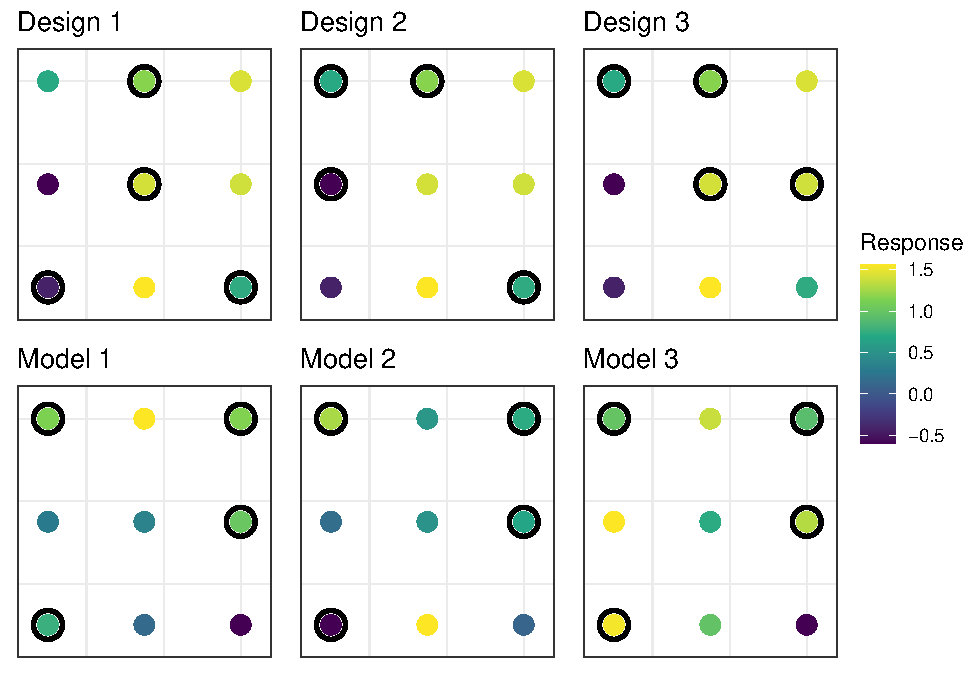
\includegraphics[width=1\linewidth]{manuscript_files/figure-latex/fig1-1} \caption{A comparison of sampling under the design-based and model-based frameworks. Points circled are those that are sampled. In the top row, we have one fixed population, and three random samples of size four. The response values at each site are fixed, but we obtain different estimates for the mean response because the randomly sampled sites vary from sample to sample. In the bottom row, we have three realizations of the same spatial process sampled at the same locations. The spatial process generating the response values has a single mean, but the realized mean is different in each of the three panels.}\label{fig:fig1}
\end{figure}

\hypertarget{subsec:spb_design}{%
\subsection{Spatially Balanced Design and
Analysis}\label{subsec:spb_design}}

The design-based approach can be used to select samples that are
``well-spread'' in space, or spatially balanced. Spatially balanced
samples are useful because parameter estimates from these samples tend
to vary less than parameter estimates from samples that are not
spatially balanced (Barabesi and Franceschi, 2011; Benedetti et al.,
2017; Grafström and Lundström, 2013; Robertson et al., 2013; Stevens and
Olsen, 2004; Wang et al., 2013). The first spatially balanced sampling
algorithm that saw widespread use was the Generalized Random
Tessellation Stratified (GRTS) algorithm (Stevens and Olsen, 2004). To
quantify the spatial balance of a sample, Stevens and Olsen (2004)
proposed loss metrics based on Voroni polygons. After the GRTS algorithm
was developed, several other spatially balanced sampling algorithms have
emerged, including the Local Pivotal Method (Grafström et al., 2012;
Grafström and Matei, 2018), Spatially Correlated Poisson Sampling
(Grafström, 2012), Balanced Acceptance Sampling (Robertson et al.,
2013), Within-Sample-Distance Sampling (Benedetti and Piersimoni, 2017),
and Halton Iterative Partitioning Sampling (Robertson et al., 2018). In
this manuscript, we use the Generalized Random Tessellation Stratified
(GRTS) algorithm to select spatially balanced samples sampling because
the algorithm has several attractive properties. It accommodates finite
and infinite sampling frames. It accommodates equal, unequal, and
proportional (to size) inclusion probabilities. It accommodates legacy
(historical) sampling (Foster et al., 2017). It accommodates a minimum
distance between units in a sample. Lastly, it accommodates replacement
units in a sample, which are units that can be sampled in place of an
original unit that can no longer be sampled. The GRTS algorithm samples
from finite and infinite populations by utilizing a mapping between
two-dimensional and one-dimensional space. The units in the
two-dimensional sampling frame are divided into cells using a
hierarchical address. This hierarchical address is then used to map the
units from two-dimensional space to a one-dimensional line where each
unit's line length equals its inclusion probability. A systematic sample
is conducted on the line and linked back to a unit in two-dimensional
space, which results in the desired sample. Stevens and Olsen (2004)
provides further details.

After selecting a spatially balanced sample using the GRTS algorithm
(i.e., a GRTS sample), data are collected and used to estimate
population parameters. To unbiasedly estimate population means and
totals from sample data, one can use the Horvitz-Thompson estimator
(Horvitz and Thompson, 1952). If \(\tau\) is a population total, the
Horvitz-Thompson estimate of \(\tau\), denoted by \(\hat{\tau}_{ht}\),
is is given by \begin{align}\label{eq:ht}
  \hat{\tau}_{ht} = \sum_{i = 1}^n Z_i \pi_i^{-1},
\end{align} where \(Z_i\) is the value of the \(i\)th unit in the sample
and \(\pi_i\) is the inclusion probability of the \(i\)th unit in the
sample. An estimate of the population mean can be obtained by dividing
\(\hat{\tau}_{ht}\) by number of population units.

While the Horvitz-Thompson estimator is unbiased for population means
and totals, it is also important to quantify the uncertainty in these
estimates. Horvitz and Thompson (1952) and Sen (1953) provide variance
estimators for \(\hat{\tau}_{ht}\), but these estimators have two
drawbacks. First, they rely on calculating \(\pi_{ij}\), the probability
that unit \(i\) and unit \(j\) are both in the sample -- this quantity
can be challenging if not impossible to calculate analytically. Second,
these estimators ignore the spatial locations of the units in the
sampling frame. To address these two drawbacks simultaneously, Stevens
and Olsen (2003) proposed the local neighborhood variance estimator. The
local neighborhood variance estimator does not rely on \(\pi_{ij}\) and
incorporates spatial locations -- for technical details see Stevens and
Olsen (2003). Stevens and Olsen (2003) show the local neighborhood
variance estimator tends to reduce the estimated variance of
\(\hat{\tau}\) compared to variance estimators ignoring spatial
locations, yielding narrower confidence intervals for \(\tau\).

\hypertarget{finite-population-block-kriging}{%
\subsection{Finite Population Block
Kriging}\label{finite-population-block-kriging}}

Finite Population Block Kriging (FPBK) is a model-based approach that
expands the geostatistical Kriging framework to the finite population
setting (Ver Hoef, 2008). Instead of developing inference based on a
specific sampling design, we assume the data are generated by a spatial
process. Ver Hoef (2008) gives details on the theory of FPBK, but some
of the basic principles are summarized below. Let
\({\mathbf{z} \equiv \{\text{z}(s_1), \text{z}(s_2), . . . , \text{z}(s_N) \}}\)
be an \(N \times 1\) response vector at locations \(s_1\), \(s_2\), . .
. , \(s_N\) that can be measured at the \(N\) population units. Suppose
we want to predict some linear function of the response variable,
\(f(\mathbf{z}) = \mathbf{b}^\prime \mathbf{z}\), where
\(\mathbf{b}^\prime\) is a \(1 \times N\) vector of weights. For
example, if we want to predict the population total across all
population units, then we would use a vector of 1's for the weights.

We often only have a sample of the \(N\) population units. Denoting
quantities that are part of the sampled population units with a
subscript \emph{s} and quantities that are part of the unsampled
population units with subscript \emph{u}, let

\begin{equation}
\begin{pmatrix} \label{equation:Zmarginal}
    \mathbf{z}_s      \\
    \mathbf{z}_u
\end{pmatrix}
=
\begin{pmatrix}
  \mathbf{X}_s    \\
  \mathbf{X}_u
\end{pmatrix}
\bm{\beta} +
\begin{pmatrix}
\bm{\delta}_s    \\
\bm{\delta}_u
\end{pmatrix},
\end{equation} where \(\mathbf{X}_s\) and \(\mathbf{X}_u\) are the
design matrices for the sampled and unsampled population units,
respectively, and \(\bm{\beta}\) is the parameter vector of fixed
effects.

Let \(\bm{\delta} \equiv [\bm{\delta}_s \,\, \bm{\delta}_u]'\), where
\(\bm{\delta}_s\) and \(\bm{\delta}_u\) are random errors for teh
sampled and unsampled population units, respectively. We assume
\(E(\bm{\delta} = \mathbf{0}\) and that there is spatial correlation in
\(\bm{\delta}\) that can be modeled using a covariance function. It is
common to assume the covariance function is second-order stationary and
isotropic (Cressie, 1993), and that the spatial covariance decreases as
the separation between population units increases. Many spatial
covariance functions exist, but the primary function we use throughout
the simulations and applications in this manuscript is the exponential
covariance function: the \(i,j\)th elment of hte matrix
\(\mathop{\mathrm{{cov}}}(\bm{\delta})\) is \mbox{}
\begin{align}\label{equation:expcov}
\mathop{\mathrm{{cov}}}(\delta_i, \delta_j) = 
\begin{cases} 
\sigma^2_{1}\exp(-h_{i,j}/\phi) & h_{i,j} > 0 \\
\sigma^2_{1} + \sigma^2_2 & h_{i,j} = 0
\end{cases}
,
\end{align} where \(\sigma^2_{1}\) is dependent random error variance
measuring coarse-scale (correlated) variability, \(\sigma^2_{2}\) is the
independent random error variance measuring fine-scale (independent)
variability, \(\phi\) is the range parameter measuring the
distance-decay rate of the correlation, and \(h_{i,j}\) is the Euclidean
distance between population units \(i\) and \(j\). Often
\(\sigma^2_{1}\) and \(\sigma^2_{2}\) are called the partial sill and
nugget, respectively. Any spatial covariance function could be used in
the place of the exponential, including functions that allow for
non-stationarity or anisotropy (Chiles and Delfiner, 1999, pp. 80--93).

With the above model formulation, the Best Linear Unbiased Predictor
(BLUP) for \(f(\mathbf{b}'\mathbf{z})\) and its prediction variance can
be computed. While details of the derivation are in (Ver Hoef, 2008), we
note here that the predictor and its variance are both moment-based,
meaning that they do not rely on any distributional assumptions.

We note that we only use FPBK in this paper in order to focus more on
comparing the design-based and model-based approaches. Other methods,
such as k-nearest-neighbors (Fix and Hodges, 1989; Ver Hoef and
Temesgen, 2013), random forest (Breiman, 2001), Bayesian models
(Chan-Golston et al., 2020), among others, could also be used to obtain
predictions for a mean or total from spatially correlated responses of a
finite population. We choose to use FPBK because it is faster than a
Bayesian approach and it was developed with theoretically-based variance
estimators of means and totals for spatial data, whereas random forests
and k-nearest-neighbors use ad-hoc variance estimators in most cases
(Ver Hoef and Temesgen, 2013); additionally, FBPK outperformed the other
methods in most scenarios.

\hypertarget{sec:numstudy}{%
\section{Numerical Study}\label{sec:numstudy}}

We used a simulation study to investigate performance of four
sampling-analysis combinations: IRS-Design, IRS with a design-based
analysis; IRS-Model, IRS with a model-based analysis; GRTS-Design, GRTS
sampling with a design-based analysis; and GRTS-Model, GRTS sampling
with a model-based analysis. These combinations are also provided in
Table \ref{tab:designanalysis}.

\begin{table}[ht]
\centering
\begin{tabular}{r|ll}
  \hline
 & Design & Model \\ 
  \hline
IRS & IRS-Design & IRS-Model \\ 
  GRTS & GRTS-Design & GRTS-Model \\ 
   \hline
\end{tabular}
\caption{\label{tab:designanalysis} Sampling-analysis combinations in the simulation study. The rows give the two types of sampling designs and the columns give the two types of analyses.} 
\end{table}

Performance of the four sampling-analysis combinations was evaluated in
36 different simulation scenarios. The 36 scenarios resulted from the
crossing of three sample sizes, two location layouts, two response
types, and three proportions of dependent random error. The three sample
sizes (\(n\)) were \(n = 50, n = 100,\) and \(n = 200\). Samples were
always selected from a population size (\(N\)) of \(N = 900\). The two
location layouts were random and gridded. Locations in the random layout
were selected randomly from the unit square (\([0, 1] \times [0, 1]\)).
Locations in the gridded layout were selected randomly on a fixed grid
from the unit square. The two response types were normal and lognormal.
For the normal response type, the response was simulated using mean-zero
random errors with the exponential covariance
(Equation\(~\)\ref{equation:expcov}) for varying proportions of
dependent random error. The proportion of dependent random error is
represented by \(\sigma^2_1 / (\sigma^2_1 + \sigma^2_2)\), where
\(\sigma^2_1\) and \(\sigma^2_2\) are from
Equation\(~\)\ref{equation:expcov}. The total variance,
\(\sigma^2_1 + \sigma^2_2\), was always 2. The range was always
\(\sqrt{2} / 3\), which means that the correlation in the dependent
random error decayed to nearly zero at the largest possible distance
between two units in the domain. For the lognormal response type, the
response was first simulated using the same approach as for the normal
response type, except that the total variance was 0.6931 instead of 2.
The response was then exponentiated, yielding a random variable whose
total variance is 2. The lognormal responses were used to evaluate
performance of the sampling-analysis approaches for data that were
skewed.

\begin{table}[ht]
\centering
\begin{tabular}{r|lll}
   \hline
Sample Size (n) & 50 & 100 & 200 \\ 
  Location Layout & Random & Gridded & - \\ 
  Proportion of Dependent Error & 0 & 0.5 & 0.9 \\ 
  Response Type & Normal & Lognormal & - \\ 
   \hline
\end{tabular}
\caption{\label{tab:parmtab} Simulation scenario options. All combinations of sample size, location layout, response type, and proportion of dependent random error composed the 36 simulation scenarios. In each simualtion scenario, the total variance was two.} 
\end{table}

In each of the 36 simulation scenarios, there were 2000 independent
simulation trials. In each trial, IRS and GRTS samples were selected and
then design-based and model-based analyses were used to estimate the
mean and construct confidence (design-based) or prediction (model-based)
intervals. We recorded the bias, squared error, and interval coverage
for all sampling-analysis combinations in each trial. Then we summarized
the performance of the combinations across trials by calculating average
bias, rMS(P)E (root-mean-squared error for the design-based approaches
and root-mean-squared-prediction error for the model-based approaches),
and the rate at which the true mean is contained in its 95\% interval.
The GRTS algorithm and the local neighborhood variance estimator are
available in the \textbf{\textsf{R}} package \texttt{spsurvey} (Dumelle
et al., 2021). FPBK is available in the \texttt{sptotal}
\textbf{\textsf{R}} package (Higham et al., 2021) and covariance
parameters were estimated using Restricted Maximum Likelihood (Harville,
1977; Patterson and Thompson, 1971; Wolfinger et al., 1994).

The average bias was nearly zero for all four combinations in all 36
scenarios, so we omit a more detailed summary of those results here.
Tables for average bias in all 36 simulation scenarios are provided in
the supplementary material.

Figure \ref{fig:figeff} shows the relative rMS(P)E of the four
approaches from Table \ref{tab:designanalysis} using the random location
layout with ``IRS-Design'' is the baseline. More formally, the relative
rMS(P)E is defined as \begin{equation*}
\frac{\text{rMS(P)E of sampling-analysis combination}}{\text{rMS(P)E of IRS-Design}},
\end{equation*} When there is no spatial correlation (Figure
\ref{fig:figeff}, top row), the four sampling-analysis combinations have
approximately equal rMS(P)E. So, using GRTS or using a spatial model
does not result in much, if any, loss in efficiency even when the
response variable is not spatially correlated. When there is spatial
correlation (Figure \ref{fig:figeff}, middle and bottom row), the
GRTS-Model combination tends to perform best, followed by GRTS-Design,
IRS-Model, and finally IRS-Design, though the difference in relative
rMS(P)E among IRS-Model, GRTS-Design, and GRTS-Model is relatively
small. As the strength of spatial correlation increases, the gap in
rMS(P)E between IRS-Design and the other combinations widens. Finally we
note that when there is spatial correlation, IRS-Model outperforms
IRS-Design by a large margin, suggesting that the poor design properties
of IRS are largely mitigated by the model-based analysis. These
conclusions are similar to those observed in the grid location layout.
Tables for rMS(P)E in all 36 simulation scenarios are provided in the
supplementary material.

\begin{figure}
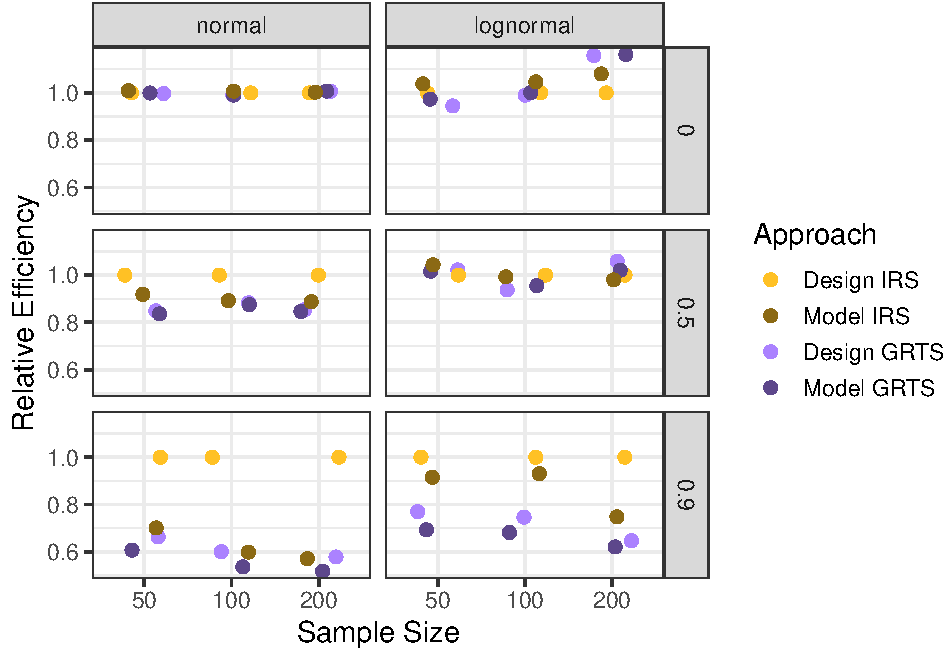
\includegraphics[width=1\linewidth]{manuscript_files/figure-latex/figeff-1} \caption{Relative rMS(P)E for the four sampling-analysis combinations. The rows indicate the proportion of dependent error and the columns indicate the response type.}\label{fig:figeff}
\end{figure}

We also studied 95\% interval coverage among the combinations. The
design-based 95\% confidence intervals and model-based 95\% prediction
intervals were constructed using the normal distribution. Justification
for the design-based and model-based intervals comes from the asymptotic
normality of totals via the Central Limit Theorem.

Figure \ref{fig:figconf} shows the 95\% interval coverage for each of
the four combinations in the random location layout. All four
combinations have fairly similar interval coverage within each scenario.
Coverage in the normal response scenarios tended to be near 95\% and
slightly higher than coverage in the lognormal scenarios. Coverage in
the lognormal scenarios still generally exceeded 90\%. Coverage tended
to always increase with the sample size. At a sample size of 200, all
four combinations had approximately 95\% interval coverage in both
response scenarios and all dependent error proportions. These
conclusions were similar to those found in the grid location layout.
Tables for interval coverage in all 36 simulation scenarios are provided
in the supplementary material.

\begin{figure}
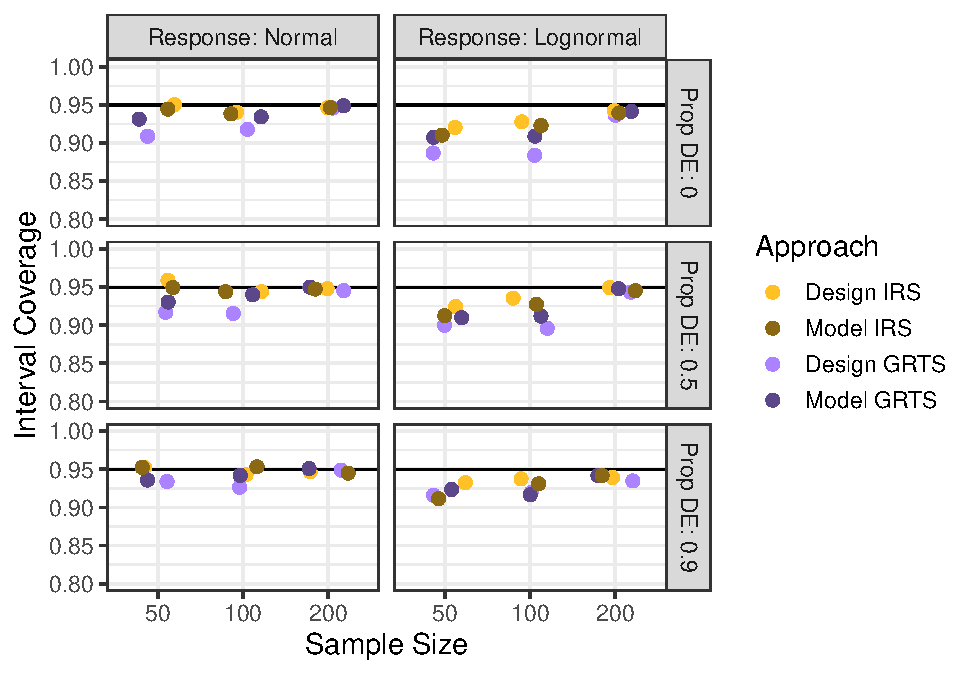
\includegraphics[width=1\linewidth]{manuscript_files/figure-latex/figconf-1} \caption{Interval coverage for the four sampling-analysis combinations. The rows indicate the proportion of dependent error and the columns indicate the response type. The solid, black line in each plot represents 95\% coverage.}\label{fig:figconf}
\end{figure}

\hypertarget{application}{%
\section{Application}\label{application}}

The Environmental Protection Agency (EPA), states, and tribes
periodically conduct National Aquatic Research Surveys (NARS) in the
United States to assess the water quality of various bodies of water. We
will use the 2012 National Lakes Assessment (NLA), which measures
various aspects of lake health and quality in lakes in the contiguous
United States, to study mercury concentration. Although we know the true
mean mercury concentration values for the 986 lakes from the 2012 NLA,
we will explore whether or not we obtain an adequately precise estimate
for the realized mean mercury concentration if we sample only 100 of the
986 lakes.

Figure \ref{fig:figdata} shows that mercury concentration is
right-skewed, with most lakes having a low value of mercury
concentration but a few having a much higher concentration. Mercury
concentration exhibits some spatial correlation, with high mercury
concentrations in lakes in the northeast and north central United
States. The realized mean mercury concentration in the 986 lakes is
103.2 ng / g.

\begin{figure}

{\centering 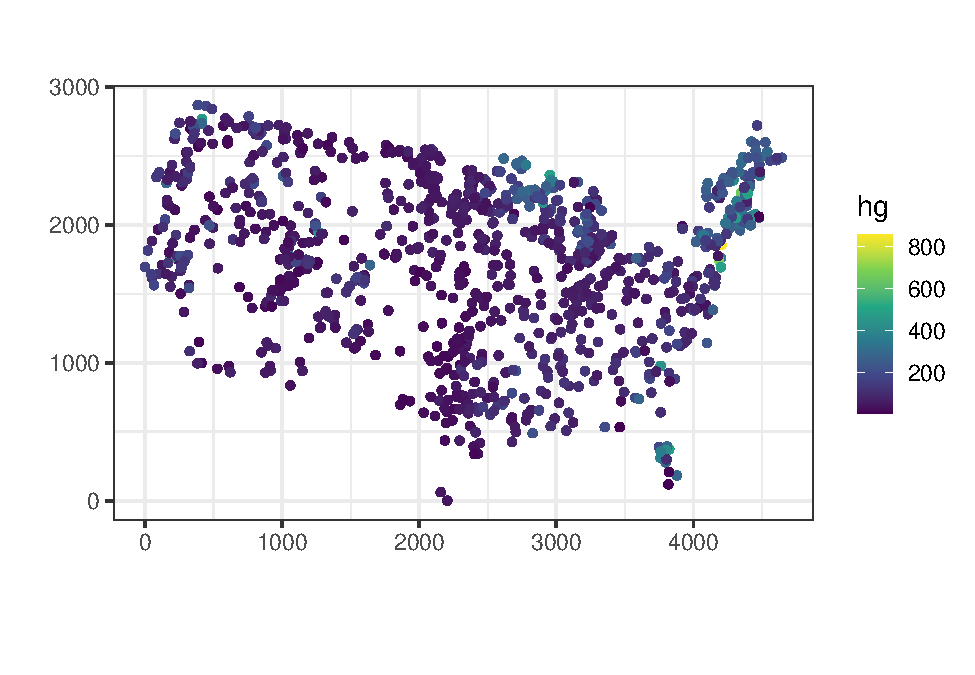
\includegraphics[width=0.49\linewidth]{manuscript_files/figure-latex/figdata-1} 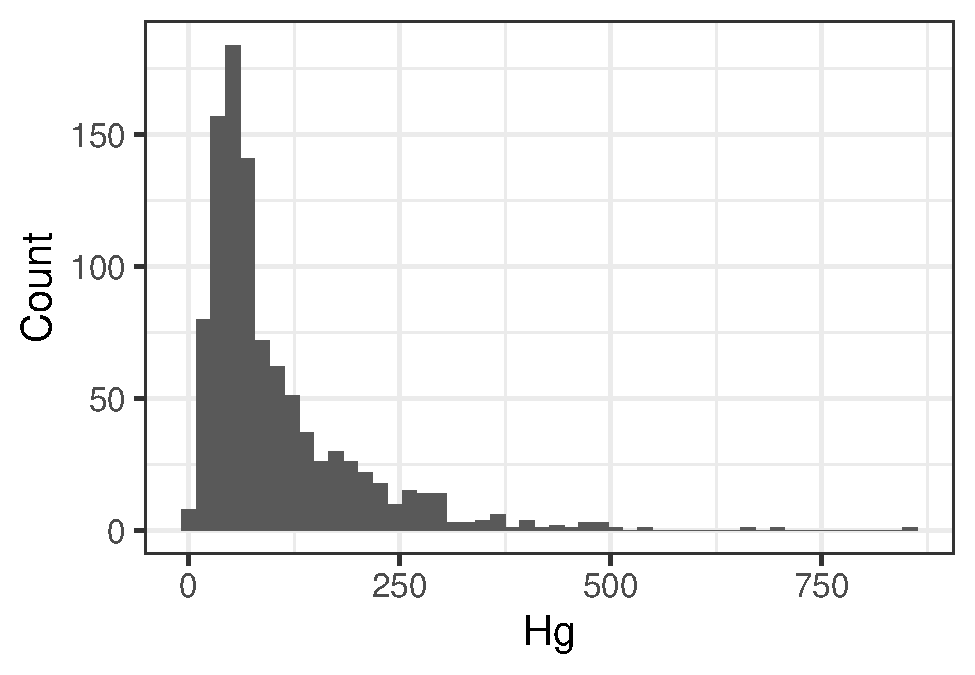
\includegraphics[width=0.49\linewidth]{manuscript_files/figure-latex/figdata-2} 

}

\caption{Population distribution of mercury concentration (hg) for 986 lakes in the contiguous United States in a spatial layout (left) and a histogram (right).}\label{fig:figdata}
\end{figure}

\begin{table}[ht]
\centering
\begin{tabular}{lrrrr}
  \hline
Approach & Estimate & SE & 95\% LB & 95\% UB \\ 
  \hline
IRS-Design & 112.7 & 8.8 & 95.4 & 129.9 \\ 
  IRS-Model & 110.5 & 7.9 & 95.0 & 125.9 \\ 
  GRTS-Design & 101.8 & 6.1 & 89.8 & 113.7 \\ 
  GRTS-Model & 102.3 & 5.9 & 90.8 & 113.9 \\ 
   \hline
\end{tabular}
\caption{\label{tab:appliedtab} Application of design-based and model-based approaches to the NLA data set on mercury concentration. The true mean concentration is 103.2 ng / g.} 
\end{table}

We selected a single IRS sample and a single GRTS sample and estimated
the mean mercury concentration and its standard error using using
design-based and model-based approaches; Table \ref{tab:appliedtab}
shows the results. For all four sampling-analysis combinations, the true
realized mean mercury concentration is within the bounds of the 95\%
intervals. However, we should not generalize these results to any other
data or even to other samples from these data. But, we do note a couple
of patterns. The design-based IRS analysis shows the largest standard
error: a likely reason is that this is the only approach that does not
incorporate any spatial information regarding mercury concentration
across the contiguous United States. We also see that both approaches
using the GRTS sample have a lower standard error than the both
approaches using the IRS sample. We would expect this to be the case for
most samples because mercury concentration exhibits spatial patterning,
so a spatially balanced sample should usually yield a lower standard
error.

To better understand the dependence structure in mercury concentration,
the empirical semivariogram and corresponding fit of the model-based
approaches can be visualized. The empirical semivariogram quantifies the
halved squared differences (semivariance) among response values at
different distances apart. If a process exhibits strong spatial
dependence, the empirical semivariogram will have small values at small
distances and large values at large distances. Figure \ref{fig:figsv}
shows the empirical semivariogram for GRTS-Model, displaying the average
semivariance for several distances. Overlain onto Figure \ref{fig:figsv}
is the estimated semivariance obtained using the covariance parmaeters
from the REML fit of GRTS-Model. Figure \ref{fig:figsv} provides
evidence that there is strong correlation in mercury concentration among
the sites.

\begin{figure}

{\centering 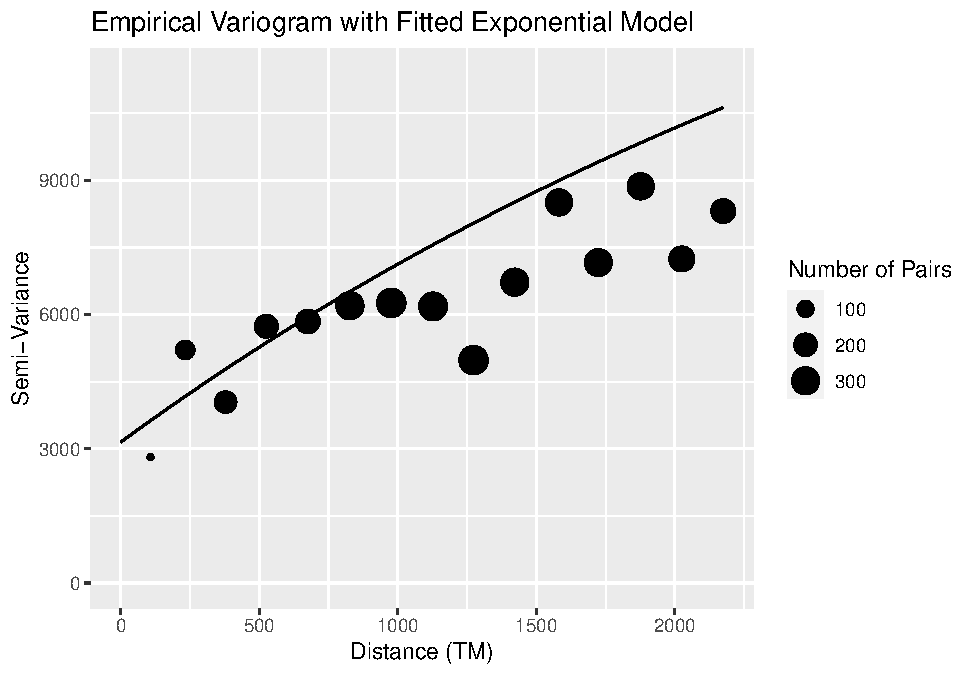
\includegraphics[width=0.85\linewidth]{manuscript_files/figure-latex/figsv-1} 

}

\caption{The empirical semivariogram (black circles) of mercury concentration against the REML fit using the estimated covariance parameters (black line) from GRTS-Model.}\label{fig:figsv}
\end{figure}

\hypertarget{sec:discussion}{%
\section{Discussion}\label{sec:discussion}}

The design-based and model-based approaches to inference are
fundamentally different paradigms by which samples are selected and data
are analyzed. The design-based approach incorporates randomness through
sampling to estimate a population parameter. The model-based approach
incorporates randomness through distributional assumptions to predict
the realized values of a random process. Though these approaches have
often been compared in the literature both from theoretical and
analytical perspectives, our contribution lies in studying them in a
spatial context while implementing spatially balanced sampling. Aside
from the theoretical differences described, a few analytical findings
from the simulation study are particularly notable. First, the sampling
decision (GRTS vs IRS) is most important when using a design-based
analysis. Though GRTS-Model still outperformed IRS-Model, the
model-based analysis mitigated much of the inefficiency of the IRS
sample. Second, independent of the analysis approach, there is no reason
to use IRS over GRTS for sampling spatial data, as GRTS-Design and
GRTS-Model generally performed at least as well as their IRS
counterparts when there was no spatial correlation and noticeably better
than there IRS counterparts when there was spatial correlation. Third,
The stronger the spatial correlation, the larger the gap in rMS(P)E
between IRS-Design and the other sampling-analysis combinations. Fourth
and finally, interval coverage for the normal response was very close to
95\% for all sample sizes, while interval coverage for the lognormal
response was not very close to 95\% until \(n = 200\).

There are several benefits and drawbacks of the design-based and
model-based approaches for spatial data, some of which we have not yet
discussed but are worthy of consideration in future research.
Design-based approaches are often computationally efficient, while
model-based estimation of covariance parameters can be computationally
burdensome, especially for likelihood-based methods such as REML that
rely on inverting a covariance matrix. The design-based approach also
more naturally handles binary data, free from the more complicated
logistic regression formulation commonly used to handle binary data in a
model-based approach. The model-based approach, however, can more
naturally quantify the relationship between covariates (predictor
variables) and the response variable. The model-based approach also
yields estimated spatial covariance parameters, which help better
understand the process of study. Model selection is also possible using
model-based approaches and criteria such as cross validation, likelihood
ratio tests, or AIC (Akaike, 1974). Model-based approaches are capable
of more efficient small-area estimation than design-based approaches by
leveraging distributional assumptions in areas with few observed sites.
Model-based approaches can also compute site-by-site predictions at
unobserved locations and use them to construct informative
visualizations. The benefits and drawbacks of both approaches, alongside
our theoretical and analytical comparisons, should be seriously
considered when choosing among them. This is especially true from an
analysis perspective, as we found that using a spatially balanced
sampling algorithm benefits both design-based and model-based analyses.

\hypertarget{data-and-code-availability}{%
\section*{Data and Code Availability}\label{data-and-code-availability}}
\addcontentsline{toc}{section}{Data and Code Availability}

This manuscript has a supplementary R package that contains all of the
data and code used. Instructions for download at available at
\url{https://github.com/michaeldumelle/DvMsp}.

\hypertarget{supplementary-material}{%
\section*{Supplementary Material}\label{supplementary-material}}
\addcontentsline{toc}{section}{Supplementary Material}

In the supplementary material, we provide tables presenting summary
statistics for all 36 simulation scenarios.

\hypertarget{references}{%
\section*{References}\label{references}}
\addcontentsline{toc}{section}{References}

\hypertarget{refs}{}
\begin{CSLReferences}{1}{0}
\leavevmode\hypertarget{ref-akaike1974new}{}%
Akaike, H., 1974. A new look at the statistical model identification.
IEEE Transactions on Automatic Control 19, 716--723.

\leavevmode\hypertarget{ref-barabesi2011sampling}{}%
Barabesi, L., Franceschi, S., 2011. Sampling properties of spatial total
estimators under tessellation stratified designs. Environmetrics 22,
271--278.

\leavevmode\hypertarget{ref-benedetti2017spatially}{}%
Benedetti, R., Piersimoni, F., 2017. A spatially balanced design with
probability function proportional to the within sample distance.
Biometrical Journal 59, 1067--1084.

\leavevmode\hypertarget{ref-benedetti2017spatiallyreview}{}%
Benedetti, R., Piersimoni, F., Postiglione, P., 2017. Spatially balanced
sampling: A review and a reappraisal. International Statistical Review
85, 439--454.

\leavevmode\hypertarget{ref-breiman2001random}{}%
Breiman, L., 2001. Random forests. Machine Learning 45, 5--32.

\leavevmode\hypertarget{ref-brus1997random}{}%
Brus, D., De Gruijter, J., 1997. Random sampling or geostatistical
modelling? Choosing between design-based and model-dased sampling
strategies for soil (with discussion). Geoderma 80, 1--44.

\leavevmode\hypertarget{ref-brus2021statistical}{}%
Brus, D.J., 2021. Statistical approaches for spatial sample survey:
Persistent misconceptions and new developments. European Journal of Soil
Science 72, 686--703.

\leavevmode\hypertarget{ref-chan2020bayesian}{}%
Chan-Golston, A.M., Banerjee, S., Handcock, M.S., 2020. Bayesian
inference for finite populations under spatial process settings.
Environmetrics 31, e2606.

\leavevmode\hypertarget{ref-chiles1999geostatistics}{}%
Chiles, J.-P., Delfiner, P., 1999. Geostatistics: {Modeling Spatial
Uncertainty}. {John Wiley \& Sons}, New York.

\leavevmode\hypertarget{ref-cicchitelli2012model}{}%
Cicchitelli, G., Montanari, G.E., 2012. Model-assisted estimation of a
spatial population mean. International Statistical Review 80, 111--126.

\leavevmode\hypertarget{ref-cooper2006sampling}{}%
Cooper, C., 2006. Sampling and variance estimation on continuous
domains. Environmetrics 17, 539--553.

\leavevmode\hypertarget{ref-cressie1993statistics}{}%
Cressie, N., 1993. Statistics for spatial data. John Wiley \& Sons.

\leavevmode\hypertarget{ref-de1990model}{}%
De Gruijter, J., Ter Braak, C., 1990. Model-free estimation from spatial
samples: A reappraisal of classical sampling theory. Mathematical
Geology 22, 407--415.

\leavevmode\hypertarget{ref-diggle2010geostatistical}{}%
Diggle, P.J., Menezes, R., Su, T., 2010. Geostatistical inference under
preferential sampling. Journal of the Royal Statistical Society: Series
C (Applied Statistics) 59, 191--232.

\leavevmode\hypertarget{ref-dumelle2021spsurvey}{}%
Dumelle, M., Kincaid, T.M., Olsen, A.R., Weber, M.H., 2021. Spsurvey:
Spatial sampling design and analysis.

\leavevmode\hypertarget{ref-fix1989discriminatory}{}%
Fix, E., Hodges, J.L., 1989. Discriminatory analysis. Nonparametric
discrimination: Consistency properties. International Statistical
Review/Revue Internationale de Statistique 57, 238--247.

\leavevmode\hypertarget{ref-foster2017spatially}{}%
Foster, S.D., Hosack, G.R., Lawrence, E., Przeslawski, R., Hedge, P.,
Caley, M.J., Barrett, N.S., Williams, A., Li, J., Lynch, T., others,
2017. Spatially balanced designs that incorporate legacy sites. Methods
in Ecology and Evolution 8, 1433--1442.

\leavevmode\hypertarget{ref-grafstrom2012spatiallypoisson}{}%
Grafström, A., 2012. Spatially correlated poisson sampling. Journal of
Statistical Planning and Inference 142, 139--147.

\leavevmode\hypertarget{ref-grafstrom2013well}{}%
Grafström, A., Lundström, N.L., 2013. Why well spread probability
samples are balanced. Open Journal of Statistics 3, 36--41.

\leavevmode\hypertarget{ref-grafstrom2012spatially}{}%
Grafström, A., Lundström, N.L., Schelin, L., 2012. Spatially balanced
sampling through the pivotal method. Biometrics 68, 514--520.

\leavevmode\hypertarget{ref-grafstrom2018spatially}{}%
Grafström, A., Matei, A., 2018. Spatially balanced sampling of
continuous populations. Scandinavian Journal of Statistics 45, 792--805.

\leavevmode\hypertarget{ref-hansen1983evaluation}{}%
Hansen, M.H., Madow, W.G., Tepping, B.J., 1983. An evaluation of
model-dependent and probability-sampling inferences in sample surveys.
Journal of the American Statistical Association 78, 776--793.

\leavevmode\hypertarget{ref-harville1977maximum}{}%
Harville, D.A., 1977. Maximum likelihood approaches to variance
component estimation and to related problems. Journal of the American
Statistical Association 72, 320--338.

\leavevmode\hypertarget{ref-higham2021sptotal}{}%
Higham, M., Ver Hoef, J., Frank, B., Dumelle, M., 2021. Sptotal:
Predicting totals and weighted sums from spatial data.

\leavevmode\hypertarget{ref-horvitz1952generalization}{}%
Horvitz, D.G., Thompson, D.J., 1952. A generalization of sampling
without replacement from a finite universe. Journal of the American
Statistical Association 47, 663--685.

\leavevmode\hypertarget{ref-lohr2009sampling}{}%
Lohr, S.L., 2009. Sampling: Design and analysis. Nelson Education.

\leavevmode\hypertarget{ref-patterson1971recovery}{}%
Patterson, H.D., Thompson, R., 1971. Recovery of inter-block information
when block sizes are unequal. Biometrika 58, 545--554.

\leavevmode\hypertarget{ref-robertson2013bas}{}%
Robertson, B., Brown, J., McDonald, T., Jaksons, P., 2013. BAS: Balanced
acceptance sampling of natural resources. Biometrics 69, 776--784.

\leavevmode\hypertarget{ref-robertson2018halton}{}%
Robertson, B., McDonald, T., Price, C., Brown, J., 2018. Halton
iterative partitioning: Spatially balanced sampling via partitioning.
Environmental and Ecological Statistics 25, 305--323.

\leavevmode\hypertarget{ref-sarndal2003model}{}%
Särndal, C.-E., Swensson, B., Wretman, J., 2003. Model assisted survey
sampling. Springer Science \& Business Media.

\leavevmode\hypertarget{ref-schabenberger2017statistical}{}%
Schabenberger, O., Gotway, C.A., 2017. Statistical methods for spatial
data analysis. CRC press.

\leavevmode\hypertarget{ref-sen1953estimate}{}%
Sen, A.R., 1953. On the estimate of the variance in sampling with
varying probabilities. Journal of the Indian Society of Agricultural
Statistics 5, 127.

\leavevmode\hypertarget{ref-sterba2009alternative}{}%
Sterba, S.K., 2009. Alternative model-based and design-based frameworks
for inference from samples to populations: From polarization to
integration. Multivariate Behavioral Research 44, 711--740.

\leavevmode\hypertarget{ref-stevens2003variance}{}%
Stevens, D.L., Olsen, A.R., 2003. Variance estimation for spatially
balanced samples of environmental resources. Environmetrics 14,
593--610.

\leavevmode\hypertarget{ref-stevens2004spatially}{}%
Stevens, D.L., Olsen, A.R., 2004. Spatially balanced sampling of natural
resources. Journal of the American Statistical Association 99, 262--278.

\leavevmode\hypertarget{ref-verhoef2002sampling}{}%
Ver Hoef, J., 2002. Sampling and geostatistics for spatial data.
Ecoscience 9, 152--161.

\leavevmode\hypertarget{ref-verhoef2008spatial}{}%
Ver Hoef, J.M., 2008. Spatial methods for plot-based sampling of
wildlife populations. Environmental and Ecological Statistics 15, 3--13.

\leavevmode\hypertarget{ref-ver2013comparison}{}%
Ver Hoef, J.M., Temesgen, H., 2013. A comparison of the spatial linear
model to nearest neighbor (k-NN) methods for forestry applications. PlOS
ONE 8, e59129.

\leavevmode\hypertarget{ref-wang2013design}{}%
Wang, J.-F., Jiang, C.-S., Hu, M.-G., Cao, Z.-D., Guo, Y.-S., Li, L.-F.,
Liu, T.-J., Meng, B., 2013. Design-based spatial sampling: Theory and
implementation. Environmental Modelling \& Software 40, 280--288.

\leavevmode\hypertarget{ref-wang2012review}{}%
Wang, J.-F., Stein, A., Gao, B.-B., Ge, Y., 2012. A review of spatial
sampling. Spatial Statistics 2, 1--14.

\leavevmode\hypertarget{ref-wolfinger1994computing}{}%
Wolfinger, R., Tobias, R., Sall, J., 1994. Computing gaussian
likelihoods and their derivatives for general linear mixed models. SIAM
Journal on Scientific Computing 15, 1294--1310.

\end{CSLReferences}


\end{document}
